\documentclass[9pt,aspectratio=169,xcolor=table]{beamer}

%~~~~~~~~~~~~~~~~~~~~~~~~~~~~~~~~~~~~~~~~~~~~~~~~~~~~~~~~~~~~~~~~~~~~~~~~~~~~~~
% Use roboto Font (recommended)
\usepackage[sfdefault]{roboto}
\usepackage[utf8]{inputenc}
\usepackage[T1]{fontenc}
%~~~~~~~~~~~~~~~~~~~~~~~~~~~~~~~~~~~~~~~~~~~~~~~~~~~~~~~~~~~~~~~~~~~~~~~~~~~~~~

%~~~~~~~~~~~~~~~~~~~~~~~~~~~~~~~~~~~~~~~~~~~~~~~~~~~~~~~~~~~~~~~~~~~~~~~~~~~~~~
% Define where theme files are located. ('/styles')
\usepackage{styles/fluxmacros}
\usefolder{styles}
% Use Flux theme v0.1 beta
% Available style: asphalt, blue, red, green, gray
\usetheme[style=gray]{flux}
%~~~~~~~~~~~~~~~~~~~~~~~~~~~~~~~~~~~~~~~~~~~~~~~~~~~~~~~~~~~~~~~~~~~~~~~~~~~~~~

%~~~~~~~~~~~~~~~~~~~~~~~~~~~~~~~~~~~~~~~~~~~~~~~~~~~~~~~~~~~~~~~~~~~~~~~~~~~~~~
% Extra packages
\usepackage{booktabs}
\usepackage{colortbl}
\usepackage{ragged2e}
\usepackage{amssymb}
\usepackage{multirow}
\usepackage{tikz}
\usetikzlibrary{arrows.meta, positioning, fit, backgrounds, calc, decorations.pathreplacing}
\setbeamertemplate{itemize items}[square]
\usepackage[scaled=.8]{beramono}
\usepackage{listings}
\usepackage{styles/lstlangarm}
\usepackage{array}
\definecolor{bgcolor}{HTML}{F2E9E9}
% lstlangarm.sty references \color{mauve} for string literals but never defines
% it -- only fires when a listing contains a string. Define it here.
\definecolor{mauve}{rgb}{0.58,0,0.82}
% lstlangarm's C style sets commentstyle=green!20, which is unreadable on the
% pink listing background. Darken it globally.
\lstset{commentstyle=\color{green!45!black}}
% ragged-right fixed-width column -- must be defined in the preamble, never
% inside a frame (\newcolumntype's #1 breaks beamer's frame scanner)
\newcolumntype{R}[1]{>{\RaggedRight\arraybackslash}p{#1}}
%~~~~~~~~~~~~~~~~~~~~~~~~~~~~~~~~~~~~~~~~~~~~~~~~~~~~~~~~~~~~~~~~~~~~~~~~~~~~~~
% Table striping: odd rows white, even rows very light gray.
% Needs \documentclass[...,xcolor=table]{beamer} (beamer loads xcolor itself,
% so the option must go on the class, not \usepackage).
\definecolor{stripe}{gray}{0.94}
% \striped makes body rows alternate white, gray, white, ... starting white.
% \rowcolors counts from the first coloured body row; the header is not counted.
\newcommand{\striped}{\rowcolors{1}{white}{stripe}}
%~~~~~~~~~~~~~~~~~~~~~~~~~~~~~~~~~~~~~~~~~~~~~~~~~~~~~~~~~~~~~~~~~~~~~~~~~~~~~~

%~~~~~~~~~~~~~~~~~~~~~~~~~~~~~~~~~~~~~~~~~~~~~~~~~~~~~~~~~~~~~~~~~~~~~~~~~~~~~~
% TikZ block styles -- matches ch1/ch2
% Colour variables are named identically in the book's stm32primer.tex, so any
% tikzpicture using only the \tikzset{...} styles below can be copied verbatim
% between slides and book. Only the \definecolor/\colorlet VALUES differ: the
% book is printed, so it keeps every stroke pure black with muted fills. These
% slides are projected, so both fill AND stroke are bright and saturated to
% grab attention -- see stm32primer.tex for the print palette.
\definecolor{blkfill}{HTML}{DCEBFF}
\definecolor{blkline}{HTML}{1565C0}
\definecolor{accentfill}{HTML}{FFE0B2}
\definecolor{accentline}{HTML}{E65100}
\definecolor{memfill}{HTML}{DFF5DA}
\definecolor{memline}{HTML}{2E7D32}
\definecolor{cellfill}{HTML}{FFFFFF}
\definecolor{cellline}{HTML}{424242}
\definecolor{bitmaskfill}{HTML}{DCEBFF}
\definecolor{bitmaskline}{HTML}{1565C0}
\definecolor{bithitfill}{HTML}{FFE0B2}
\definecolor{bithitline}{HTML}{E65100}
\tikzset{
  blk/.style   = {rectangle, rounded corners=2pt, draw=blkline, fill=blkfill,
                  thick, align=center, font=\small, minimum height=9mm, inner sep=3pt},
  cpublk/.style= {rectangle, rounded corners=2pt, draw=accentline, fill=accentfill,
                  thick, align=center, font=\small\bfseries, minimum height=9mm, inner sep=3pt},
  memblk/.style= {rectangle, rounded corners=2pt, draw=memline, fill=memfill,
                  thick, align=center, font=\small, minimum height=9mm, inner sep=3pt},
  cell/.style  = {rectangle, draw=cellline, fill=cellfill, align=center,
                  font=\small\ttfamily, minimum height=7mm, inner sep=2pt},
  lbl/.style   = {font=\scriptsize, text=Gray},
  flow/.style  = {-{Stealth[length=2mm]}, thick, draw=blkline},
  busline/.style={thick, draw=cellline},
}
% NOTE (theme quirks -- all fail SILENTLY, always page through the PDF):
%  - a second \\ inside a nested {...} group in a TikZ node breaks parsing
%  - {\small ...} wrapped around a nested itemize eats the frame title + list
%  - \usebeamercolor on a [plain] frame falls through to an unstyled default
%  - \newcolumntype inside a frame breaks beamer's frame scanner
%  - lstlisting needs \begin{frame}[fragile]
%  - a TikZ picture wider than its column silently overflows into neighbours
%~~~~~~~~~~~~~~~~~~~~~~~~~~~~~~~~~~~~~~~~~~~~~~~~~~~~~~~~~~~~~~~~~~~~~~~~~~~~~~

%%%%%%%%%%%%%%%%%%%%%%%%%%%%%%%%%%%
%% BEGIN CONDITIONAL COMPILATION %%
%%%%%%%%%%%%%%%%%%%%%%%%%%%%%%%%%%%
\newif\ifwebex
%\webextrue % uncomment to generate section separator
\ifwebex
\AtBeginSection[]{
  \begin{frame}
  \vfill
  \centering
  \begin{beamercolorbox}[sep=8pt,center,shadow=true,rounded=true]{title}
    \usebeamerfont{title}\insertsectionhead\par%
  \end{beamercolorbox}
  \vfill
  \end{frame}
}
\else
\AtBeginSection[]
{
{
    \setbeamercolor{background canvas}{bg=yellow!10}
    \begin{frame}[plain]
        \frametitle{Table of Contents}
        \tableofcontents[currentsection]
    \end{frame}
}
}
\fi
%%%%%%%%%%%%%%%%%%%%%%%%%%%%%%%%%%%
%% END CONDITIONAL COMPILATION   %%
%%%%%%%%%%%%%%%%%%%%%%%%%%%%%%%%%%%

%~~~~~~~~~~~~~~~~~~~~~~~~~~~~~~~~~~~~~~~~~~~~~~~~~~~~~~~~~~~~~~~~~~~~~~~~~~~~~~
% Information
\title{ADC and Analog Interfacing}
\subtitle{\emph{Introduction to ARM Cortex-M Microprocessors} --- Chapter 11}
\author{Mun\'{i}m Zabidi}
\institute{\color{primary}Faculty of Electrical Engineering, Universiti Teknologi Malaysia}
\date{\today}
\titlegraphic{assets/logoutmwhite.png}
%~~~~~~~~~~~~~~~~~~~~~~~~~~~~~~~~~~~~~~~~~~~~~~~~~~~~~~~~~~~~~~~~~~~~~~~~~~~~~~

\begin{document}

\titlepage

%===============================================================================
\section{Why This Matters}
%===============================================================================

\begin{frame}{Why This Chapter Matters}
    \begin{columns}[T]
    \begin{column}{.47\textwidth}
        {\normalsize Temperature, light, sound and force are continuous. A processor works only with numbers. The ADC crosses that gap. Using it well is an engineering problem: how fast to sample, how much resolution you need, and how much of the answer you can trust.}
    \end{column}
    \begin{column}{.51\textwidth}
        \begin{block}{After this chapter, you can:}
        {\small
        \begin{enumerate}\itemsep2pt
            \item Explain sampling, quantization and resolution; apply Nyquist.
            \item Calculate the step size and convert codes to volts.
            \item Configure a pin for analog input and set up the ADC.
            \item Read by polling and by interrupt.
            \item Choose the sampling time for a source impedance.
            \item Scale a raw reading into engineering units.
        \end{enumerate}}
        \end{block}
    \end{column}
    \end{columns}
\end{frame}


%===============================================================================
\section{Sampling and Resolution}
%===============================================================================

\begin{frame}{Two Approximations at Once}
    \begin{columns}[T]
    \begin{column}{.48\textwidth}
        \textbf{Sampling} --- discrete in \alert{time}

        \vspace{1mm}
        {\small You measure at instants, not continuously. Between samples, the
        signal is unknown.}

        \vspace{2mm}
        {\small \textbf{Nyquist:} sample at more than \alert{twice} the highest
        frequency present, or the reconstruction is wrong.}
    \end{column}
    \begin{column}{.48\textwidth}
        \textbf{Quantization} --- discrete in \alert{value}

        \vspace{1mm}
        {\small Each sample becomes one of a finite set of numbers. 12 bits gives
        $2^{12} = 4096$ levels, \alert{0 to 4095}.}

        \vspace{2mm}
        {\small The error is up to half a step --- inherent, not a defect.}
    \end{column}
    \end{columns}

    \vspace{3mm}
    \begin{block}{Aliasing is not recoverable}
        Sample a 600\,Hz tone at 1\,kHz and it reappears as 400\,Hz --- and no
        amount of later processing can tell it from a real 400\,Hz signal. The
        fix is an \alert{anti-alias filter in hardware}, before the ADC.
    \end{block}
\end{frame}

\begin{frame}{From Count to Voltage}
    \begin{center}
    \fbox{\parbox{.6\textwidth}{\centering\vspace{1mm}
    $V_{\text{in}} = \dfrac{\text{count}}{4095} \times V_{\text{ref}}$
    \vspace{1mm}}}
    \end{center}

    \vspace{3mm}
    \begin{center}
    {\small
    \striped
    \begin{tabular}{@{}l l l@{}}
        \toprule
        \textbf{Count} & \textbf{Voltage} ($V_{\text{ref}} = 3.3$\,V) & \textbf{Meaning} \\
        \midrule
        \texttt{0}    & 0.00\,V  & Input at ground \\
        \texttt{1}    & 0.81\,mV & \alert{One step} --- the smallest detectable change \\
        \texttt{2048} & 1.65\,V  & Half scale \\
        \texttt{4095} & 3.30\,V  & Full scale \\
        \bottomrule
    \end{tabular}}
    \end{center}

    \vspace{3mm}
    \begin{block}{Resolution is a voltage, not a bit count}
        ``12-bit'' sounds abstract. What it \emph{means} is that the smallest
        change you can see is $3.3 / 4095 \approx \alert{0.8\,\text{mV}}$.
        Anything finer is invisible to your program.
    \end{block}
\end{frame}

%===============================================================================
\section{Using the ADC}
%===============================================================================

\begin{frame}[fragile]{Configuration}
\begin{lstlisting}[language=C, basicstyle=\ttfamily\scriptsize]
// 1. Clocks
RCC->AHB1ENR |= (1U << 0);      // GPIOA
RCC->APB2ENR |= (1U << 8);      // ADC1

// 2. PA0 as analog -- MODER bits 11, the fourth mode from Chapter 8
GPIOA->MODER |= (3U << 0);

// 3. Sampling time: 480 cycles on channel 0
ADC1->SMPR2 |= (7U << 0);

// 4. Sequence: one conversion, channel 0
ADC1->SQR1 = 0;                 // L = 0 means 1 conversion
ADC1->SQR3 = 0;                 // first in sequence is channel 0

// 5. Turn it on
ADC1->CR2 |= (1U << 0);         // ADON
\end{lstlisting}

    \vspace{1mm}
    {\small On this course \texttt{PA0} is \texttt{ADC1} channel \texttt{0} ---
    and note \texttt{MODER} $=$ \texttt{11}, the analog mode that has been waiting
    since Chapter 8.}
\end{frame}

\begin{frame}[fragile]{Reading a Value}
    \begin{columns}[T]
    \begin{column}{.52\textwidth}
\begin{lstlisting}[language=C, basicstyle=\ttfamily\scriptsize]
uint16_t ADC_Read(void)
{
    ADC1->CR2 |= (1U << 30);   // SWSTART
    while (!(ADC1->SR & (1U << 1)))
        ;                      // wait for EOC
    return ADC1->DR;           // reading DR
}                              // clears EOC
\end{lstlisting}
    \end{column}
    \begin{column}{.44\textwidth}
        \begin{enumerate}
            \item \alert{Start} --- set \texttt{SWSTART}
            \item \alert{Wait} --- poll \texttt{EOC}
            \item \alert{Read} --- \texttt{DR} holds the result, and reading it
                  clears the flag
        \end{enumerate}
    \end{column}
    \end{columns}

    \vspace{3mm}
    \begin{block}{This blocks, and Chapter 9 said why that is a shame}
        The processor does nothing during the conversion. A real design uses the
        \alert{end-of-conversion interrupt}, or lets \alert{DMA} move the result
        with no CPU involvement at all.
    \end{block}
\end{frame}

\begin{frame}{Sampling Time}{The setting people get wrong}
    \begin{columns}[T]
    \begin{column}{.5\textwidth}
        \begin{itemize}
            \item The ADC charges an internal capacitor from your signal
                  \alert{before} converting.
            \item \alert{Sampling time} is how long it is given to charge ---
                  3 to 480 cycles.
        \end{itemize}

        \vspace{2mm}
        {\ttfamily\scriptsize ADC1->SMPR2 |= (7U << 0);~// 480 cycles}
    \end{column}
    \begin{column}{.46\textwidth}
        \begin{block}{Too short, and you read nonsense}
            A \alert{high-impedance} source --- a potentiometer, a sensor behind a
            large resistor --- charges that capacitor slowly. Convert too early and
            you measure a \emph{partly charged} capacitor, not your signal.
        \end{block}
    \end{column}
    \end{columns}

    \vspace{3mm}
    {\small The symptom is characteristic: readings \alert{consistently low}, or
    changing when you touch the wiring. The fix is a longer sampling time --- or a
    buffer amplifier.}
\end{frame}

\begin{frame}{From Codes to Engineering Units}
    \begin{columns}[T]
    \begin{column}{.5\textwidth}
        \textbf{A thermocouple amplifier}

        \vspace{1mm}
        {\small Outputs 0--3.3\,V for 0--400\,\textdegree C.}

        \vspace{2mm}
        {\ttfamily\scriptsize
        float volts = (raw * 3.3f) / 4095.0f; \\
        float degC~ = volts * (400.0f / 3.3f);}

        \vspace{2mm}
        {\small Or in one step:}

        \vspace{1mm}
        {\ttfamily\scriptsize float degC = raw * (400.0f / 4095.0f);}
    \end{column}
    \begin{column}{.46\textwidth}
        \begin{block}{Can you actually resolve 1\,\textdegree C?}
            400\,\textdegree C over 4096 steps is
            \alert{0.098\,\textdegree C per step} --- ten times better than
            needed.

            \vspace{2mm}
            So the ADC is not your limit. \alert{Noise} is --- and that is an
            analog design problem, not a programming one.
        \end{block}
    \end{column}
    \end{columns}

    \vspace{2mm}
    {\small Note the \texttt{f} suffixes: \texttt{3.3f} is a \texttt{float};
    plain \texttt{3.3} is a \texttt{double}, which the Cortex-M4's FPU
    \alert{cannot} do in hardware.}
\end{frame}

\begin{frame}{Resolution Is Not Accuracy}
    \leavevmode
    \begin{columns}[T]
    \begin{column}{.48\textwidth}
        \begin{block}{Resolution}
            {\small The smallest change the ADC can \alert{tell apart}.}

            \vspace{1mm}
            {\small 12-bit: $3.3/4096 \approx 0.8$~mV.}
        \end{block}

        \vspace{2mm}
        {\small A property of the \alert{bit count}. It never gets
        better than this.}
    \end{column}
    \begin{column}{.48\textwidth}
        \begin{block}{Accuracy}
            {\small How close the reading is to the \alert{true} voltage.}

            \vspace{1mm}
            {\small Set by reference tolerance, offset, gain error,
            noise, source impedance, sampling time.}
        \end{block}

        \vspace{2mm}
        {\small Can be far worse than resolution. 12-bit numbers do
        not guarantee 12-bit answers.}
    \end{column}
    \end{columns}

    \vspace{3mm}
    \begin{block}{Averaging}
        $N$ independent samples reduce random noise by $\sqrt{N}$.
        Trades conversion rate for a quieter number.
    \end{block}
\end{frame}

\begin{frame}{An Analog Measurement at Five Levels}
    \begin{center}
    {\small
    \striped
    \begin{tabular}{@{}l R{.65\textwidth}@{}}
        \toprule
        \textbf{Level} & \textbf{Representation} \\
        \midrule
        Physical    & 1.599~V on the PA0 pad from the potentiometer wiper \\
        Hardware    & Sample-and-hold capacitor; 12-cycle SAR comparison \\
        Register    & \texttt{ADC1->DR} contains \texttt{0x7C0} \\
        C           & \texttt{voltage = raw * 3.3f / 4095.0f;} \\
        Engineering & 1.599~V, or 159.9~\textdegree{}C from an LM35 \\
        \bottomrule
    \end{tabular}}
    \end{center}

    \vspace{3mm}
    \begin{block}{What the ADC gives you}
        A continuous quantity sensed through a chain that starts at a
        physical voltage and ends in engineering units. With a hardware
        timer driving conversions, the interval is set by the peripheral,
        not by the main loop.
    \end{block}
\end{frame}

\begin{frame}{Summary}
	\begin{columns}[c]
		\begin{column}{.62\textwidth}
			\begin{center}
				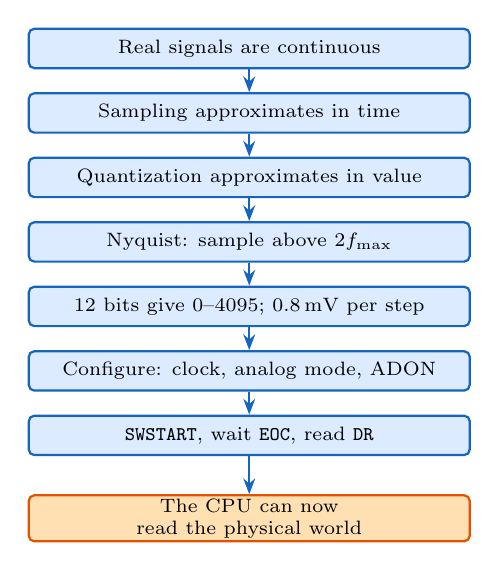
\begin{tikzpicture}[x=10mm, y=7.8mm]
					\node[blk, minimum width=56mm, minimum height=5.0mm, inner sep=1.2pt, font=\scriptsize] (n0) at (0,0.00) {Real signals are continuous};
					\node[blk, minimum width=56mm, minimum height=5.0mm, inner sep=1.2pt, font=\scriptsize] (n1) at (0,-1.05) {Sampling approximates in time};
					\node[blk, minimum width=56mm, minimum height=5.0mm, inner sep=1.2pt, font=\scriptsize] (n2) at (0,-2.10) {Quantization approximates in value};
					\node[blk, minimum width=56mm, minimum height=5.0mm, inner sep=1.2pt, font=\scriptsize] (n3) at (0,-3.15) {Nyquist: sample above $2f_{\max}$};
					\node[blk, minimum width=56mm, minimum height=5.0mm, inner sep=1.2pt, font=\scriptsize] (n4) at (0,-4.20) {12 bits give 0--4095; 0.8\,mV per step};
					\node[blk, minimum width=56mm, minimum height=5.0mm, inner sep=1.2pt, font=\scriptsize] (n5) at (0,-5.25) {Configure: clock, analog mode, ADON};
					\node[blk, minimum width=56mm, minimum height=5.0mm, inner sep=1.2pt, font=\scriptsize] (n6) at (0,-6.30) {\texttt{SWSTART}, wait \texttt{EOC}, read \texttt{DR}};
					\node[cpublk, minimum width=56mm, minimum height=5.0mm, inner sep=1.2pt, font=\scriptsize, align=center] (n7) at (0,-7.65) {The CPU can now\\read the physical world};
					\foreach \a/\b in {0/1,1/2,2/3,3/4,4/5,5/6,6/7}{\draw[flow] (n\a) -- (n\b);}
				\end{tikzpicture}
			\end{center}
		\end{column}
		\begin{column}{.34\textwidth}
			{\scriptsize
				\textbf{Terminology covered}\\[1mm]
				\begin{itemize}
					\item Sampling, quantization
					\item Nyquist, aliasing
					\item Resolution, step size
					\item Sampling time, impedance
					\item \texttt{EOC}, \texttt{DR}
				\end{itemize}
				\vspace{3mm}
				\textbf{Next: Chapter 12}\\[1mm]
				\emph{UART Communication}\\[1mm]
				We can read the world. Next, we report it.}
		\end{column}
	\end{columns}
\end{frame}

\end{document}

